\documentclass[11pt]{article}

\usepackage{geometry}
\geometry{letterpaper}
\geometry{margin=1in}

\usepackage[parfill]{parskip}
\usepackage{graphicx}
\usepackage{hyperref}
\usepackage{color}
\usepackage{amssymb}

\usepackage{tcolorbox}
\tcbset{
	colback=black!2!white, colframe=black!50, arc=0mm, boxrule=0.15mm,
	left=3pt, after={\parfillskip=0pt\par},before={\parfillskip=0pt\par}}
	% - added after and removed "after skip=15pt" to avoid Overfull \hbox warnings
	% - also replace "before skip=12pt" with "before={\parfillskip=0pt\par}"
	%   because the former was not recognized on all my machines

\newcommand{\tag}[1]{{\tt #1}}
\newcommand{\attr}[1]{{\tt #1}}
\newcommand{\attrs}[1]{\{#1\}}

\newcommand{\tab}{\hspace*{1cm}}

\newcommand{\sep}{
	\begin{center}
	%\rule{40pt}{1pt}
	%$\ast \ast \ast$
	$\diamond \diamond \diamond$
	%$\divideontimes \divideontimes \divideontimes $ 
	\end{center}
}

\newenvironment{example}
    {\begin{tcolorbox}\small}
    {\end{tcolorbox}}
%\renewenvironment{example}{}{}

\newenvironment{mappings}
	{\medskip\begin{tabular}{|l|l|}\hline}
	{\hline\end{tabular}\medskip}

\newenvironment{vocabitem}
	{\begin{mappings}}
	{\end{mappings}}

\setlength{\skip\footins}{0.6cm}


\title{Mapping TCF and LIF}

\author{Marc Verhagen}

%\date{}


\begin{document}

\maketitle


\section{Introduction}
% --------------------------------------------------------------------------------------------------------

This document contains mappings of data elements of the Text Corpus Format (TCF) used by WebLicht and the LAPPS Interchange Format (LIF) used by the LAPPS Grid. The descriptions here are based on the information in:

\begin{itemize}

\item The TCF Format explained.\\
{\color{blue}\href{http://weblicht.sfs.uni-tuebingen.de/weblichtwiki/index.php/The_TCF_Format}{http://weblicht.sfs.uni-tuebingen.de/weblichtwiki/index.php/The\_TCF\_Format}}

\item The TCF schema\\
{\color{blue}\href{https://github.com/weblicht/tcf-spec/blob/master/src/main/rnc-schema/textcorpus_0_4.rnc}{https://github.com/weblicht/tcf-spec/blob/master/src/main/rnc-schema/textcorpus\_0\_4.rnc}}

\item The specifications of the LAPPS Interchange Format:
{\color{blue}\href{http://wiki.lappsgrid.org/interchange/}{http://wiki.lappsgrid.org/interchange/}}

\item The LAPPS vocabulary website:
{\color{blue}\href{http://vocab.lappsgrid.org/}{http://vocab.lappsgrid.org/}}

\end{itemize}

The mappings are provided in a series of tables and are structured around several categories (tokens, sentences, parsing, etcetera) and for each category examples of both TCF and LIF are given. But we start with some high-level observations to accompany the tables. 

First, assuming that the LAPPS vocabulary contains the categories needed to express all information in a TCF layer, then a single view can be created for each layer. The one exception is the combination of the \tag{tokens}, \tag{POStags} and \tag{lemmas} layers, which most naturally map to a single LIF view with \tag{Token} annotation types. Second, since LIF has no strict rules on what annotation types co-occur in a view, we list the most common combinations. Third, one tricky issue that may not be solved is what to do with LIF representations that contain several layers with the same annotations. For example, it is totally okay if there are two Token views, it seems like TCF has no natural way of dealing with this.

The initial description of what's involved in the mapping is centered around two simple yet not trivial use cases. The first case is of a LAPPS user who has built a pipeline of several LAPPS services followed by one WebLicht service, this is partially depicted in Figure \ref{fig:lif2tcf2lif} where we se the LIF representation as created by the LAPPS services, how that LIF representation is mapped to TCF, and then how after WebLicht processing the TCF is mapped back to LIF.

\begin{figure}[ht]
  \begin{center}
    \fbox{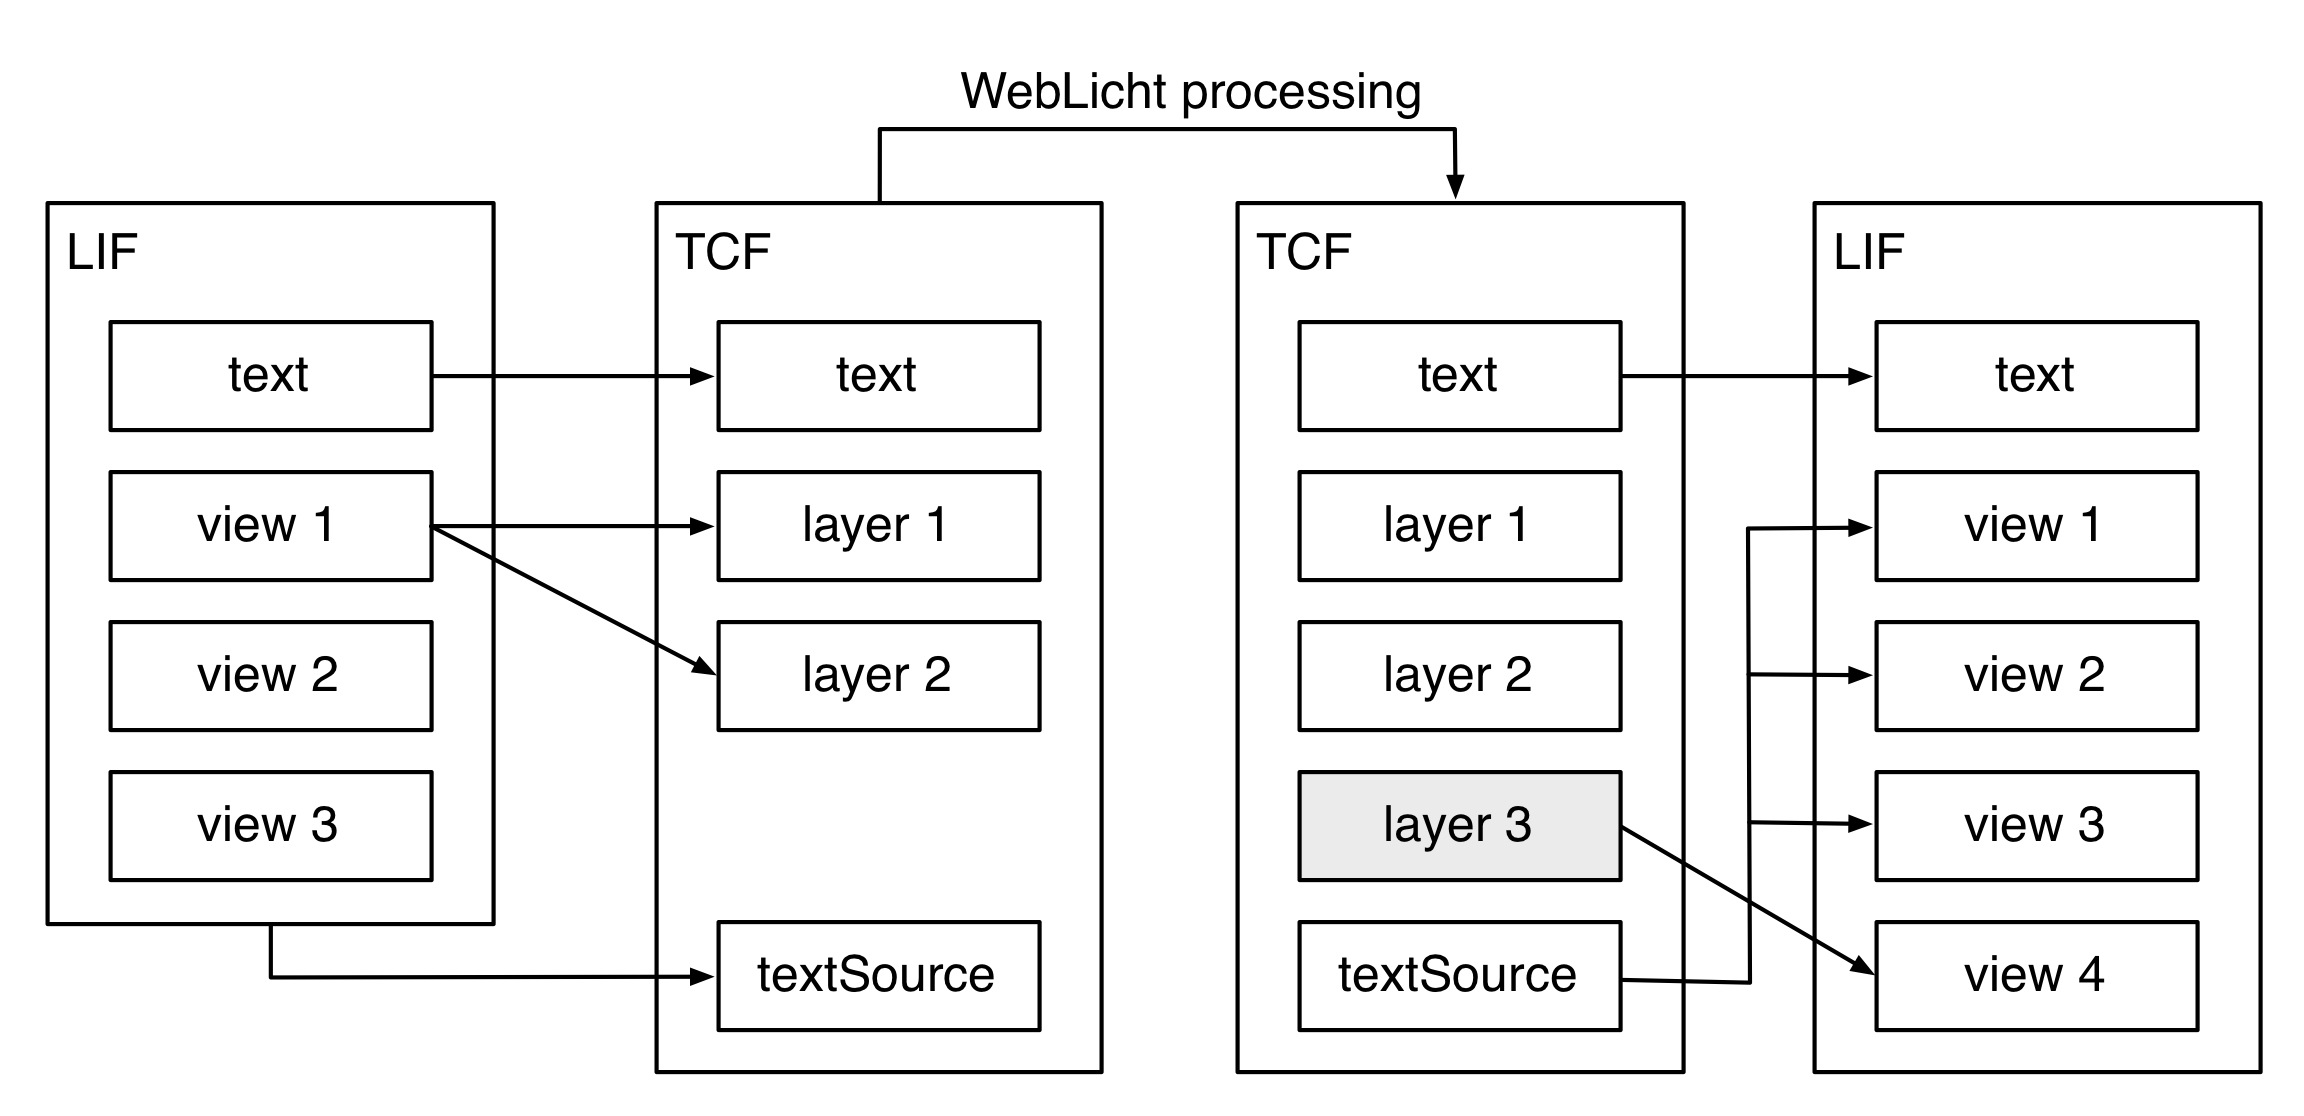
\includegraphics[width=.80\textwidth]{images/mapping-lif-tcf-lif.jpg}}
    \caption{Accessing a WebLicht service from LAPPS}
    \label{fig:lif2tcf2lif}
  \end{center}
\end{figure}

For the WebLicht service to run the LIF representation first needs to be mapped to TCF (see the left two boxes of the figure. Here are some remarks on that mapping:

\begin{enumerate}

\item The text can relatively simply be mapped from LIF to TCF since the way the text is represented in LIF and TCF is essentially the same.

\item The example here has three LIF views where one of them maps to two TCF annotation layers. This could for example be a view with Token annotations where the Tokens each have a \tag{pos} tag. In addition, there are two LIF views that have no clearly defined mapping to TCF layers or that are not needed for the processing performed by the WebLicht service.

\item The entire LIF representation has a natural landing spot in the \tag{textSource} tag in TCF (which is mostly used to store the TEI source of a document). Using this tag has the advantage that the mapping to TCF now becomes lossless. Some information in LIF views cannot naturally be expressed in TCF (character offsets for example) and having the entire LIF stored in a special field makes it possible to just transfer the information needed to use the WebLicht service.

\end{enumerate}

WebLicht processing occurs in the middle of Figure \ref{fig:lif2tcf2lif} and for the example we simply assume that just one new layer is created. The deal now with mapping back to LIF is that the original LIF views can be restored from the TCF \tag{textSource} layer. It would potentially be possible to restore view~1 from layers 1 and 2, but using \tag{textSource} is more robust. The new layer is mapped to a new view by convention. Note that it is sometimes possible to fold the new TCF layer into an existing LIF view. This if for example the case when the TCF layer is a \tag{lemmas} or \tag{POStags} layer and the LIF representation already has a Tokens view. In that case having a new view may introduce redundancy, which is a common occurrence in LIF.

The second use case is that of a WebLicht user who has built a pipeline of several WebLicht services followed by one LAPPS service. This is depicted partially in Figure \ref{fig:tcf2lif2tcf}, in a similar way to how it was done for the reverse direction in Figure \ref{fig:lif2tcf2lif}.

\begin{figure}[ht]
  \begin{center}
    \fbox{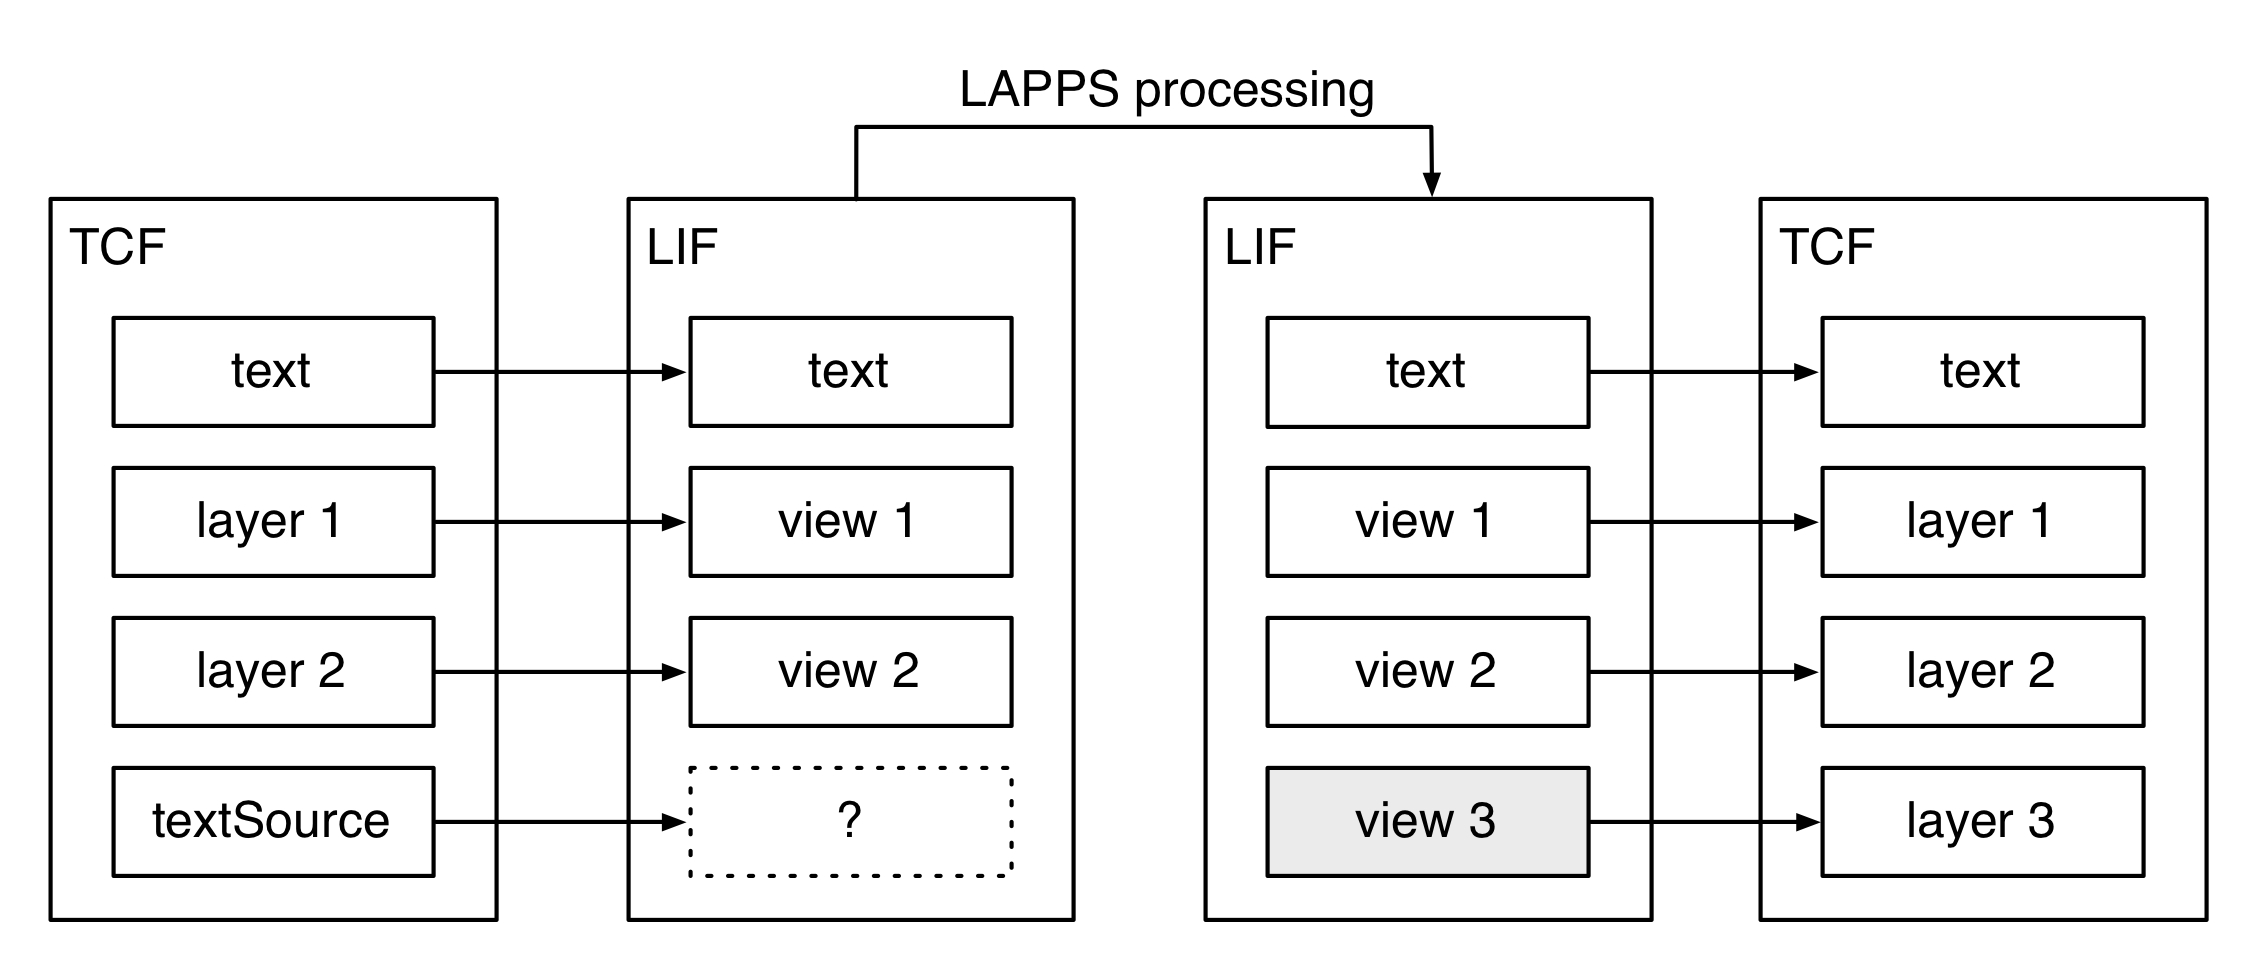
\includegraphics[width=.80\textwidth]{images/mapping-tcf-lif-tcf.jpg}}
    \caption{Accessing a LAPPS service from WebLicht}
    \label{fig:tcf2lif2tcf}
  \end{center}
\end{figure}

Here we assume that there are two TCF layers and they each happen to map to one view. We also assume that the LAPPS service used generates one new view. Technically, a LAPPS service could add annotations to an existing view, but it is recommended that services create new views and most services do that. So at this point we will not deal with those cases where existing views are updated.

The first thing to note is that LIF does not currently have the equivalent of the TCF \tag{textSource} tag so restoring the TCF layers in the right of the picture require that the mapping from layers to views is lossless. This is in most cases possible with just some changes in the LAPPS Vocabulary side of things. However, we will consider whether it is worthwhile to introduce a new structural element in LIF that can store an alternative representation.

\sep

The next sections have more details on the mappings of individual layers and views. We concentrate on the annotation contents of views and layers and have little to say about meta data. We have structured the discussion into several topics. 

For each topic we give the relevant fragments of the TCF schema and the LAPPS vocabulary as well as example TCF and LIF representations. For TCF, the concepts used are expressed in the schema, but not explicitly further semantically defined. There is the CLARIN Concept Registry at {\color{blue}\href{https://www.clarin.eu/ccr}{https://www.clarin.eu/ccr}}, but there are no explicit links from TCF to the registry. In LIF the concepts are referred to explicitly by using links to the {\color{blue}\href{http://vocab.lappsgrid.org/}{LAPPS Vocabulary}}. In our discussion we focus on changes needed to the LAPPS vocabulary and the TCF schema and we again abstract away from the problem of having to generate character offsets when we map from TCF to LIF.

At the end we summarize results for each direction in a couple of tables.


\section{Tokens, part-of-speech tags and lemmas}

While these are separate annotation layers in TCF, we group these together because on the LIF side these typically end up in the same view. First we give a TCF example for tokens and the associated schema:

\begin{example}
\begin{verbatim}
<tokens>
  <token ID="t_0">Karin</token>
  <token ID="t_1">fliegt</token>
</tokens>
\end{verbatim}
\end{example}

\begin{example}
\begin{verbatim}
tokens =
  element tokens {
    attribute charOffsets { "true" }?,
    element token {
      (attribute start { xsd:int },
       attribute end   { xsd:int })?,
      attribute ID    { xsd:ID }?,
      xsd:string
    }*
  }
\end{verbatim}
\end{example}

This layer does have an optional \attr{charOffsets} attribute which can be set to true for those cases when character offsets are available. This could be exploited by the TCF2LIF mapper, but in most cases there are no offsets alas. The \attr{ID} attribute is listed as optional, but in fact it seems to be required. 

For lemmas in TCF we have the following example and schema:

\begin{example}
\begin{verbatim}
<lemmas>
  <lemma ID="le_0" tokenIDs="t_0">Karin</lemma>
  <lemma ID="le_1" tokenIDs="t_1">fliegen</lemma>
</lemmas>
\end{verbatim}
\end{example}

\begin{example}
\begin{verbatim}
lemmas =
  element lemmas {
    element lemma {
      attribute ID    { xsd:ID }?,
      attribute tokenIDs { xsd:IDREFS },
      xsd:string
    }*
  }
\end{verbatim}
\end{example}


And finally, for part-of-speech tags we have the following.

\begin{example}
\begin{verbatim}
<POStags tagset="stts">
  <tag ID="pt_0" tokenIDs="t_0">NE</tag>
  <tag ID="pt_1" tokenIDs="t_1">VVFIN</tag>
</POStags>
\end{verbatim}
\end{example}

\begin{example}
\begin{verbatim}
POStags =
  element POStags {
    attribute tagset { xsd:string },
    element tag {
      attribute ID    { xsd:ID }?,
      attribute tokenIDs { xsd:IDREFS },
      xsd:string
    }*
  }
\end{verbatim}
\end{example}



\sep

Mapping to LIF is simple, all that is needed is to create \tag{Token} annotations in a view.

\begin{example}
\begin{verbatim}
{ "id": "v1",
  "annotations": [
    { "@type": "http://vocab.lappsgrid.org/Token",
      "id":" t_0",
      "start": 0,
      "end": 5,
      "features": { 
        "word": "Karin",
        "lemma": "Karin", "tcf_lemma_ID": "le_0",
        "pos": "NE", "tcf_POStag_ID": "pt_0" } 
    },
    { "@type": "http://vocab.lappsgrid.org/Token",
      "id":" t_1",
      "start": 6,
      "end": 11,
      "features": {
        "word": "fliegt",
        "lemma": "fliegen", "tcf_lemma_ID": "le_1",
        "pos": "VVFIN", "tcf_POStag_ID": "pt_1" } 
    }
  ]
}
\end{verbatim}
\end{example}

In both TCF and LIF the tokens are the primary thing in that lemmas and pos tags both depend on the tokens to be present. In TCF this is expressed by the lemmas pos tags referring to a token object, in LIF this is done by embedding lemmas and pos tags as attributes on a features dictionary.

The main difference is that in TCF lemmas and pos tags are first-class citizens with their own object. In LIF, all information on the lemma or pos tag needs to be copied to the Token's feature dictionary, in the example above we use \tag{tcf\_lemma\_ID} and \tag{tcf\_POStag\_ID}. Note that this does not require any changes to the LAPPS Vocabulary since it is allowed to add arbitrary features. Another difference is that in TCF a lemma or pos tag can refer to more than one token. The only way to do that in LIF is to store the attributes involved on more than one Token.
 
We now try to abstract away from the syntax of TCF and LIF and express the difference between the two notations as concept mappings. A concept mapping can be seen as linking a path in the WebLicht TCF schema to an element of the LAPPS vocabulary. Note that elements in the LAPPS vocabulary are expressed at fixed positions in a LIF representation so on the LAPPS end we can use the intended semantic for the mapping. In TCF the semantics is expressed directly and implicitly in the schema syntax, there is no explicit semantics.

In the concept mappings we use the hash symbol between concepts and their attributes, where on the TCF end these refer to elements of the schema and on the LAPPS end these refer to elements in the vocabulary. For TCF, we use \attr{cdata} as an attribute that stands for the CDATA in the XML tag. In all following tables, the first line is always the name of the TCF layer. There is no specific concept that this relates to on the LIF side, but in all cases the content of the layer is mapped to one view.

\newpage
Here are the mappings for tokens and lemmas.

\begin{mappings}
tokens				&  \\ \hline
tokens\#charOffsets & No mapping, tokens always have character offsets \\ \hline
token 				& Token \\ \hline
token\#cdata		& Token\#word \\ \hline
token\#ID 			& Token\#id \\ \hline
token\#start 		& Token\#start \\ \hline
token\#end			& Token\#end \\
\end{mappings}

% \begin{vocabitem}
% Token 				&											\\ \hline
% metadata properties 	& posTagSet, producer, rules 				\\ \hline
% inherited properties 	& alternateName, id, start, end, targets 	\\ \hline
% local properties		& pos, lemma, tokenType, orth, length, word	\\ 
% \end{vocabitem}

\begin{mappings}
lemmas			 	& \\ \hline
lemma 				& No direct mapping, attributes are embedded in Token \\ \hline
lemma\#cdata		& Token\#lemma \\ \hline
lemma\#ID 			& Token\#tcf\_lemma\_ID \\
					& In LIF lemma is an attribute that does not have its own identifier so \\
					& we park it on the Token. Syntactically this attribute is expressed in \\
					& the features dictionary. \\ \hline
lemma\#tokenIDs 	& Token\#id, but note this allows only one identifier \\
\end{mappings}

There is one things to note on the lemmas. Consider the use of \attr{tcf\_lemma\_ID}. This is an attribute that has no natural place in LIF since lemmas have no identifiers in LIF. But we do not loose it so we park it in the features dictionary of the Token and give it a special name with the \attr{tcf} prefix. We can use this for any possible feature on lemmas that do not have a LIF counter part on the Token. Note that if we have a special place in LIF to park the entire TCF representation then we would not need to do this.

Here are the concepts involved for pos tags:

\begin{mappings}
POStags			& \\ \hline
tag 			& No direct mapping, attributes are embedded in Token \\ \hline
tag\#cdata		& Token\#pos \\ \hline
tag\#ID 		& Token\#tcf\_POStag\_ID \\
				& In LIF pos is an attribute that does not have its own identifier so \\
				& we park it on the Token. Syntactically this attribute is expressed in \\
				& the features dictionary. \\ \hline
tag\#tokenIDs	& Token\#id, but note this allows only one identifier \\
\end{mappings}

The same remarks on identifiers that we had for the lemmas layer hold here as well. One difference though is that in TCF lemmas can be referred to but POStags not, so we could get away with not keeping the identifier at all.
 
The mappings above include all tags and attributes defined in TCF for the three layers. But LIF and the LAPPS Vocabulary allow arbitrary extra attributes. Changing TCF to allow for all these is not trivial and instead we will rely on the \tag{textSource} attribute (see Figure \ref{fig:lif2tcf2lif}).


\newpage
\section{Sentences}
% --------------------------------------------------------------------------------------------------------

TCF example and schema:

\begin{example}
\begin{verbatim}
<sentences>
  <sentence ID="s_0" tokenIDs="t_0 t_1 t_2 t_3 t_4 t_5"/>
</sentences>
\end{verbatim}
\end{example}

\begin{example}
\begin{verbatim}
sentences =
  element sentences {
    attribute charOffsets { "true" }?,
    element sentence {
      attribute ID    { xsd:ID }?,
      (attribute start { xsd:int },
       attribute end   { xsd:int })?,
      attribute tokenIDs   { xsd:IDREFS }
    }*
  }
\end{verbatim}
\end{example}

This is again a fairly simple mapping, but there are two ways to represent this in LIF. The first is what is used mostly by LIF services which is to give the start and end character offsets of the sentence:

\begin{example}
\begin{verbatim}
{ "id": "v4",
  "annotations": [
    { "@type": "http://vocab.lappsgrid.org/Sentence",
      "id":" s_0",
      "start": 0,
      "end": 35,
      "features": { } 
    }
  ]
}
\end{verbatim}
\end{example}

The other way is to use the \attr{targets} attribute:

\begin{example}
\begin{verbatim}
{ "id": "v4",
  "annotations": [
    { "@type": "http://vocab.lappsgrid.org/Sentence",
      "id":" s_0",
      "targets": "t_0 t_1 t_2 t_3 t_4 t_5 ",
      "features": { } 
    }
  ]
}
\end{verbatim}
\end{example}

The Token identifiers used would then either need to be expressed in the same layer or they need to refer to another layer, so instead of \attr{t\_0} we would have \attr{v1:t\_0}.

\newpage
We have the following mappings:

\begin{mappings}
sentences				& \\ \hline
sentences\#charOffsets	& No mapping, sentences can always be related to offsets \\ \hline
sentence				& Sentence \\ \hline
sentence\#ID			& Sentence\#id \\ \hline
sentence\#tokenIDs		& Sentence\#targets \\ \hline
sentence\#start 		& Sentence\#start \\ \hline
sentence\#end			& Sentence\#end \\
\end{mappings}



\section{Phrase structure parsing}
% --------------------------------------------------------------------------------------------------------

TCF example (rather simplified) and schema:

\begin{example}
\begin{verbatim}
<parsing>
  <constituent cat="NX" ID="c_9">
    <constituent cat="NE" ID="c_7" tokenIDs="t_3"/>
    <constituent cat="NE" ID="c_8" tokenIDs="t_4"/>
  </constituent>
</parsing>
\end{verbatim}
\end{example}

\begin{example}
\begin{verbatim}
parsing =
  element parsing {
    attribute tagset { xsd:string },
    element parse {
      attribute ID    { xsd:ID }?,
      constituent
    }*
  }

constituent =
  element constituent {
    attribute cat { xsd:string },
    attribute edge { xsd:string }?,
    attribute ID { xsd:ID }?,
    element cref {
        attribute constID {xsd:ID}, # target constituent ID
        attribute edge { xsd:string } # secondary edge label
    }*,
    (attribute tokenIDs { xsd:IDREFS } | constituent*)
  }
\end{verbatim}
\end{example}

The most notable characteristic of the TCF parsing layer is that dominance relations are expressed by embedding of XML tags and not by features (with the exception of constituents that immediately dominate tokens). But in a LIF representation there is no embedding of annotation objects and dominance relations have to be expressed by attributes, as shown in the following example (which is also an example where one view refers to tokens in another view).

\begin{example}
\begin{verbatim}
{
  "text": { "@value": "Sue sees herself" },
  "views": [
    { "id": "v1",
      "metadata": {
        "contains": {
          "Token": {
            "producer": "edu.brandeis.cs.lappsgrid.opennlp.Tokenizer:2.0.3",
            "type": "tokenizer:opennlp" }}},
      "annotations": [
         { "@type": "Token", "id": "tok0", "start": 0, "end": 3 },
         { "@type": "Token", "id": "tok1", "start": 4, "end": 8 },
         { "@type": "Token", "id": "tok2", "start": 9, "end": 16 }
      ]
    },
    { "id": "v2",
      "metadata": {
        "contains": {
          "PhraseStructure": {
            "producer": "edu.brandeis.cs.lappsgrid.SimpleParser:1.0.0",
            "categorySet": "ns/types/PTBcategories",
            "type": "PhraseStructure:SimpleParser" },
          "Constituent": {
            "producer": "edu.brandeis.cs.lappsgrid.SimpleParser:1.0.0",
            "categorySet": "ns/types/PTBcategories",
            "type": "PhraseStructure:SimpleParser" }}},
      "annotations": [
         { "@type": "PhraseStructure",
           "id": "phrase0",
           "start": 0,
           "end": 16,
           "features": {
              "constituents": [ "c0", "c1", "c2", "v1:tok0", "v1:tok1", "v1:tok2" ] }},
         { "@type": "Constituent", "label": "S", "id": "c0",
           "features": {
             "parent": null,
             "children": [ "c1", "c2"] } },
         { "@type": "Constituent", "label": "NP", "id": "c1",
           "features": {
             "parent": "c0",
             "children": [ "v1:tok0" ] }},
         { "@type": "Constituent", "label": "VP", "id": "c2",
           "features": {
             "parent": "c0",
             "children": [ "v1:tok1", "v1:tok2" ] }}]}]
}
\end{verbatim}
\end{example}

This difference implies that not all information relevant for mapping  from TCF to LIF can be expressed by the concept mappings.

\newpage
Here are the mappings from TCF concepts to the LAPPS Vocabulary:

\begin{mappings}
parsing					& \\ \hline
parsing\#tagset			& PhraseStructure@categorySet	\\ \hline
parse					& PhraseStructure 				\\ \hline
parse\#ID				& PhraseStructure\#id			\\ \hline
constituent 			& Constituent 					\\ \hline
constituent\#ID 		& Constituent\#id 				\\ \hline
constituent\#cat 		& Constituent\#label		 	\\ \hline
constituent\#edge 		& No mapping				 	\\ \hline
constituent\#tokenIDs 	& Constituent\#children			\\ \hline
cref 					& No mapping 					\\ \hline
cref\#constID		 	& No mapping 					\\ \hline
cref\#edge 				& No mapping 					\\ 
\end{mappings}

Note the use of the @ symbol in \tag{PhraseStructure@categorySet}, this indicates that the property is a metadata property (these too are defined in the vocabulary). The LAPPS Vocabulary has \tag{Constituent\#parent} and \tag{Constituent\#children}. These have no counter part in TCF since there are expressed by embedding (except for the constituents that directly dominate tokens). The \tag{cref} object allows a secondary edge to another constituent, which in effect turns the tree into a directed graph. These are not widely used in WebLicht services and we ignore them for now, but when needed we can most likely use one of the relation annotation types in the vocabulary.


\newpage
\section{Dependency parsing}
% --------------------------------------------------------------------------------------------------------

TCF example and schema

\begin{example}
\begin{verbatim}
 <depparsing tagset="tiger" emptytoks="false" multigovs="false">
  <parse ID="d_0">
    <dependency govIDs="t_1" depIDs="t_0" func="SB"/>
    <dependency depIDs="t_1" func="ROOT"/>
    <dependency govIDs="t_1" depIDs="t_2" func="MO"/>
    <dependency govIDs="t_4" depIDs="t_3" func="PNC"/>
    <dependency govIDs="t_2" depIDs="t_4" func="NK"/>
    <dependency govIDs="t_4" depIDs="t_5" func="--"/>
  </parse>
  <parse ID="d_1">
    <dependency govIDs="t_7" depIDs="t_6" func="SB"/>
    <dependency depIDs="t_7" func="ROOT"/>
    <dependency govIDs="t_10" depIDs="t_8" func="MO"/>
    <dependency govIDs="t_10" depIDs="t_9" func="OA"/>
    <dependency govIDs="t_7" depIDs="t_10" func="OC"/>
    <dependency govIDs="t_10" depIDs="t_11" func="--"/>
  </parse>
</depparsing>
\end{verbatim}
\end{example}

\begin{example}
\begin{verbatim}
depparsing =
  element depparsing {
    attribute tagset { xsd:string }?,
    attribute multigovs { xsd:boolean },
    attribute emptytoks { xsd:boolean },
    element parse {
      attribute ID { xsd:ID }?,
      element dependency {
        attribute func { xsd:string }?,
        attribute depIDs { xsd:IDREFS },
        attribute govIDs { xsd:IDREFS }?
       }*,
      element emptytoks {
        element emptytok {
            attribute ID { xsd:string },
             xsd:string?
          }+
      }?
    }*
  }
\end{verbatim}
\end{example}

\newpage
LIF example

\begin{example}
\begin{verbatim}
{
  "text": { "@value": "Sue sees herself" },
  "views": [
    { "id": "v1",
      "metadata": {
        "contains": {
          "Token": {
            "producer": "edu.brandeis.cs.lappsgrid.opennlp.Tokenizer:n.n.n",
            "type": "tokenizer:opennlp" }}},
      "annotations": [
         { "@type": "Token", "id": "tok0", "start": 0, "end": 3 },
         { "@type": "Token", "id": "tok1", "start": 4, "end": 8 },
         { "@type": "Token", "id": "tok2", "start": 9, "end": 16 }
      ]
    },
    { "id": "v2",
      "metadata": {
        "contains": {
          "DependencyStructure": {
            "producer": "edu.brandeis.cs.lappsgrid.SimpleDependencyParser:1.0.0",
            "dependencySet": "ns/types/StanfordDependencies",
            "type": "DependencyStructure:SimpleDependencyParser" },
          "Dependency": {
            "producer": "edu.brandeis.cs.lappsgrid.SimpleDependencyParser:1.0.0",
            "type": "DependencyStructure:SimpleDependencyParser" }}},
      "annotations": [
         { "@type": "DependencyStructure", "id": "depstructure0", "start": 0, "end": 16,
           "features": {
              "type": "basic-dependencies",
              "dependencies": [ "dep0", "dep1", "dep2" ],
        { "@type": "Dependency", "label": "ROOT", "id": "dep0",
          "features":    {
            "governor": null,
            "dependent": "v1:tok1" }},
        { "@type": "Dependency", "label": "nsubj", "id": "dep1",
          "features":    {
            "governor": "v1:tok1",
            "dependent": "v1:tok0" }},
        { "@type": "Dependency", "label": "nobj", "id": "dep2",
          "features":    {
            "governor": "v1:tok1",
            "dependent": "v1:tok2" }}]}]}]
}
\end{verbatim}
\end{example}

\newpage

Here are the mappings:

\begin{mappings}
depparsing				& \\ \hline
depparsing\#tagset		& DependencyStructure@dependencySet	\\ \hline
depparsing\#multigovs	& No mapping						\\ \hline
depparsing\#emptytoks	& No mapping						\\ \hline
parse					& DependencyStructure 				\\ \hline
parse\#ID				& DependencyStructure\#id			\\ \hline
dependency 				& Dependency 						\\ \hline
dependency\#ID 			& Dependency\#id 					\\ \hline
dependency\#func 		& Dependency\#label				 	\\ \hline
dependency\#depIDs 		& Dependency\#dependent			 	\\ \hline
dependency\#govIDs 		& Dependency\#governor				\\ \hline
emptytoks 				& No mapping 						\\ \hline
emptytok 				& No mapping 						\\ \hline
emptytok\#ID		 	& No mapping 						\\ \hline
\end{mappings}

Note that \tag{depIDs} and \tag{govIDs} are lists. These typically have one element, but if there is a second element than this would be expressed in LIF by using two \tag{Dependency} elements. The LAPPS vocabulary defines two additional properties for \tag{DependencyStructure}: \tag{dependencyType}
and \tag{dependencies}. The first is not expressed in TCF and the second is expressed structurally by the list of \tag{dependency} tags inside of the \tag{depparsing} tag.



\section{Named entities}
% --------------------------------------------------------------------------------------------------------

TCF example and schema:

\begin{example}
\begin{verbatim}
<namedEntities type="CoNLL2002">
  <entity ID="ne_0" class="PER" tokenIDs="t_0"/>
  <entity ID="ne_1" class="LOC" tokenIDs="t_3 t_4"/>
</namedEntities>
\end{verbatim}
\end{example}

\begin{example}
\begin{verbatim}
namedEntities =
  element namedEntities {
    attribute type { xsd:string },
    attribute charOffsets { "true" }?,
    element entity {
      attribute class { xsd:string },
      attribute ID    { xsd:ID }?,
      (attribute start { xsd:int },
       attribute end   { xsd:int })?,
      attribute tokenIDs { xsd:IDREFS }
    }*
  }
\end{verbatim}
\end{example}

\newpage
LIF example:

\begin{example}
\begin{verbatim}
{
  "@context": "http://vocab.lappsgrid.org/context-1.0.0.jsonld",
  "text": { "@value": "Jill sleeps." },
  "views": [
    {
      "id": "v1",
      "metadata": {
      
        "contains": {
          "http://vocab.lappsgrid.org/NamedEntity": {
            "producer":"edu.brandeis.cs.lappsgrid.stanford.corenlp.NER:2.0.3",
            "namedEntityCategorySet": "ner:stanford" }}}
      "annotations": [
         { "@type": "NamedEntity", "id": "c0", "start": 0, "end": 4,
          "features": { "category": "person", "gender": "female" } } ]
    }
  ]
}
\end{verbatim}
\end{example}

Concept mappings:

\begin{mappings}
namedEntities				& \\ \hline
namedEntities\#type			& Not sure, probably NamedEntity@namedEntityCategorySet		\\ \hline
namedEntities\#charOffsets	& No mapping, named entities are always related to offsets	\\ \hline
entity						& NamedEntity 												\\ \hline
entity\#ID					& NamedEntity\#id											\\ \hline
entity\#class 				& NamedEntity\#category								 		\\ \hline
entity\#start 				& NamedEntity\#start										\\ \hline
entity\#end 				& NamedEntity\#end											\\ \hline
entity\#tokenIDs 			& NamedEntity\#targets										\\ \hline
\end{mappings}

The WSEV \tag{NamedEntity} annotation type also has \tag{type} and\tag{gender} attributes, there are no TCF equivalents for these.


\newpage
\section{Coreference}
% --------------------------------------------------------------------------------------------------------

TCF example and schema:

\begin{example}
\begin{verbatim}
<references typetagset="BART" reltagset="TuebaDZ">
  <entity>
    <reference ID="rc_0" tokenIDs="t_0" mintokIDs="t_0" type="nam"/>
    <reference ID="rc_1" tokenIDs="t_6" mintokIDs="t_6" type="pro.per3" 
               rel="anaphoric" target="rc_0"/>
  </entity>
  <entity>
    <reference ID="rc_2" tokenIDs="t_3 t_4" mintokIDs="t_3 t_4" type="nam"/>
    <reference ID="rc_3" tokenIDs="t_8" mintokIDs="t_8" type="adv" 
               rel="anaphoric" target="rc_2"/>
  </entity>
</references>
\end{verbatim}
\end{example}

\begin{example}
\begin{verbatim}
references =
  element references {
    attribute typetagset { xsd:string }?,
    attribute reltagset { xsd:string }?,
    attribute extrefs { xsd:string }?,
    entity*
  }

entity = 
  element entity {
    attribute ID { xsd:ID }?,
    extref?,
    reference+
  }
  
extref =
  element extref {
   attribute refid { xsd:string }  
  } 

reference =
  element reference {
    attribute ID { xsd:ID }?,
    attribute rel { xsd:string }?,
    attribute target { xsd:IDREFS }?,
    attribute tokenIDs { xsd:IDREFS },
    attribute mintokIDs { xsd:IDREFS }?,
    attribute type { xsd:string }?
  }
\end{verbatim}
\end{example}

As with phrase structure parsers, some of the information is encoded in the XML tree and not on the tags themselves.

LIF has several ways of dealing with this, see {\color{blue}\href{http://wiki.lappsgrid.org/interchange/coref.html}{http://wiki.lappsgrid.org/interchange/coref.html}}, the closest to the TCF way is the following.


\begin{example}
\begin{verbatim}
{
  "text": "Sue sees herself",
  "views": [
    { "id": "v1",
       "metadata": {
        "contains": {
          "Token": {
            "producer": "edu.brandeis.cs.lappsgrid.opennlp.Tokenizer:1.1.0",
            "type": "tokenizer:opennlp" }}},
      "annotations": [
         { "@type": "Token", "id": "tok0", "start": 0, "end": 3 },
         { "@type": "Token", "id": "tok1", "start": 4, "end": 8 },
         { "@type": "Token", "id": "tok2", "start": 9, "end": 16 } ]},
    { "id": "v2",
      "metadata": {
        "contains": {
          "Markable": {
            "producer": "edu.brandeis.cs.lappsgrid.opennlp.coref:1.1.0" },
          "Coreference": {
            "producer": "edu.brandeis.cs.lappsgrid.opennlp.coref:1.1.0" }}},
      "annotations": [
         { "@type": "Markable", "id": "m0", "targets": [ "v1:tok0" ] },
         { "@type": "Markable", "id": "m1", "targets": [ "v1:tok2" ] },
         { "@type": "Coreference",
           "id": "coref0",
           "features": {
             "mentions": [ "m0", "m1" ],
             "representative": "m0" }}]}]
}
\end{verbatim}
\end{example}

Concept mappings (very incomplete):

\begin{mappings}
references				& \\ \hline
references\#typetagset	& 											\\ \hline
references\#reltagset	&											\\ \hline
references\#extrefs		& 											\\ \hline
entity					& Coreference 								\\ \hline
entity\#ID				& Coreference\#id							\\ \hline
extref\#class 			& 								 			\\ \hline
extref\#refid 			&											\\ \hline
reference 				& Markable									\\ \hline
reference\#ID 			& Markable\#id								\\ \hline
reference\#rel			& 											\\ \hline
reference\#target 		& 											\\ \hline
reference\#tokenIDs 	& Markable\#targets							\\ \hline
reference\#mintokIDs 	& 											\\ \hline
reference\#type 		& 											\\ \hline
\end{mappings}


\section{Other layers}
% --------------------------------------------------------------------------------------------------------

In TCF there are various other layers that we have left out of the discussion because in the current phase of the project we have no intention to integrate WebLicht tools that produce these layers. In many cases, these layers are not widely used within WebLicht. And, similarly, the LAPPS Vocabulary contains a few annotation types that have no equivalent in TCF. We will not go into detail on these layers and annotation types, but the summary tables in the next section do refer to them with some minor remarks.



%\section{Mapping Metadata}
% --------------------------------------------------------------------------------------------------------
%\label{sec:metadata}



\section{Summary tables of mappings between TCF and LIF/WSEV}
% --------------------------------------------------------------------------------------------------------


\input{table-tcf-lif.tex}

\medskip

\input{table-lif-tcf.tex}

%Table \ref{table:tcf2lif}
%
%\begin{table}[ht]
%\input{table-tcf-lif.tex}
%\caption{Mappings from TCF to LIF/WSEV}
%\label{table:tcf2lif}
%\end{table}
%
%Table \ref{table:lif2tcf}
%
%\begin{table}[ht]
%\input{table-lif-tcf.tex}
%\caption{Mappings from LIF/WSEV to TCF}
%\label{table:lif2tcf}
%\end{table}

\end{document}  